\subsection{Controlled Object Monitor}
Mit der \nameref{sec:controlled-object-factory} wurde festgelegt, welche Prozesse wie auf ein Objekt zugreifen dürfen. Mit dem \emph{Controlled Object Monitor} gibt es nun ein Werkzeug, wie diese Zugriffsbeschränkungen effektiv und zentral durchgesetzt werden können.

\subsection*{Kontext}
Ein Betriebssystem welches mehreren Benutzern Zugriff auf Objekte mit definierten Zugriffsbedingungen gewährt.

\subsection*{Problem}
Wie kann gewährleistet werden, dass jegliche Zugriffe auf die Objekte in einem System geprüft und ggf. abgebrochen werden, falls der zugreifende Prozess die nötigen Bedingungen nicht erfüllt?

\begin{itemize}
	\item Es gibt viele verschiedene Objekte mit verschiedensten Zugriffsberechtigungen. Jegliche Zugriffe auf sie muss kontrolliert werden
	\item Es gibt verschiedene Zugriffsarten (read, write etc.)
\end{itemize}


\subsection*{Lösung}
Durch die Verwendung eines Reference Monitors werden alle Zugriffe von Prozessen Objekte abgefangen und überprüft.

\begin{figure}[H]
	\centering
	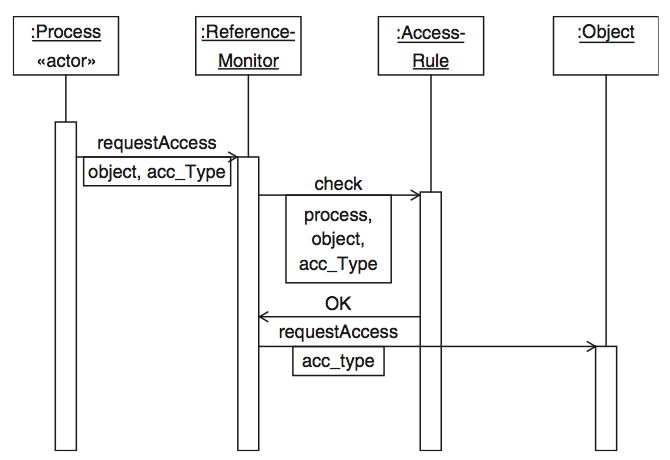
\includegraphics[width=10cm]{content/security/operating-system-access-control/images/controlled-object-monitor.png}
	\caption{Behandlung eines Zugriffs mit Controlled Object Monitor \cite{SecPatterns06}}
\end{figure}


\subsection*{Vorteile}
\begin{itemize}
	\item Jeder Zugriff eines Prozesses auf jegliche Objekte kann gem. Sicherheitsrichtlinien überprüft werden
	\item Durch Verwendung von Zugriffsmatrizen können verschiedenen Zugriffstypen definiert und gesondert geprüft werden.
	\item Inhaltsspezifische Regeln sind machbar (Achtung Performance!)
\end{itemize}

\subsection*{Nachteile}
\begin{itemize}
	\item Zugriffsberechtigungen (z.B. Zugriffsmatrizen) müssen geschützt werden! Evtl. sogar über die gleichen Mechanismen (Oh hay, deadlock.)
	\item Die Überprüfung jedes Zugriffes führt zu einem entsprechenden Overhead
\end{itemize}